\documentclass[12pt]{article}
\usepackage{todonotes,mathtools,microtype,amsfonts,amssymb,fullpage,graphicx,float, setspace}
\title{\vspace{-2cm}Design Document}
\author{Siddharth Gupta, 20823830}
\date{December 16, 2020}
\begin{document}
	\maketitle
	% \tableofcontents
	% \doublespacing
	\section{Introduction}
		For the CS246 Final Project, I chose to work on the game ``Straights,'' a single-person project.
	\section{Overview}
		\begin{figure}[H]
			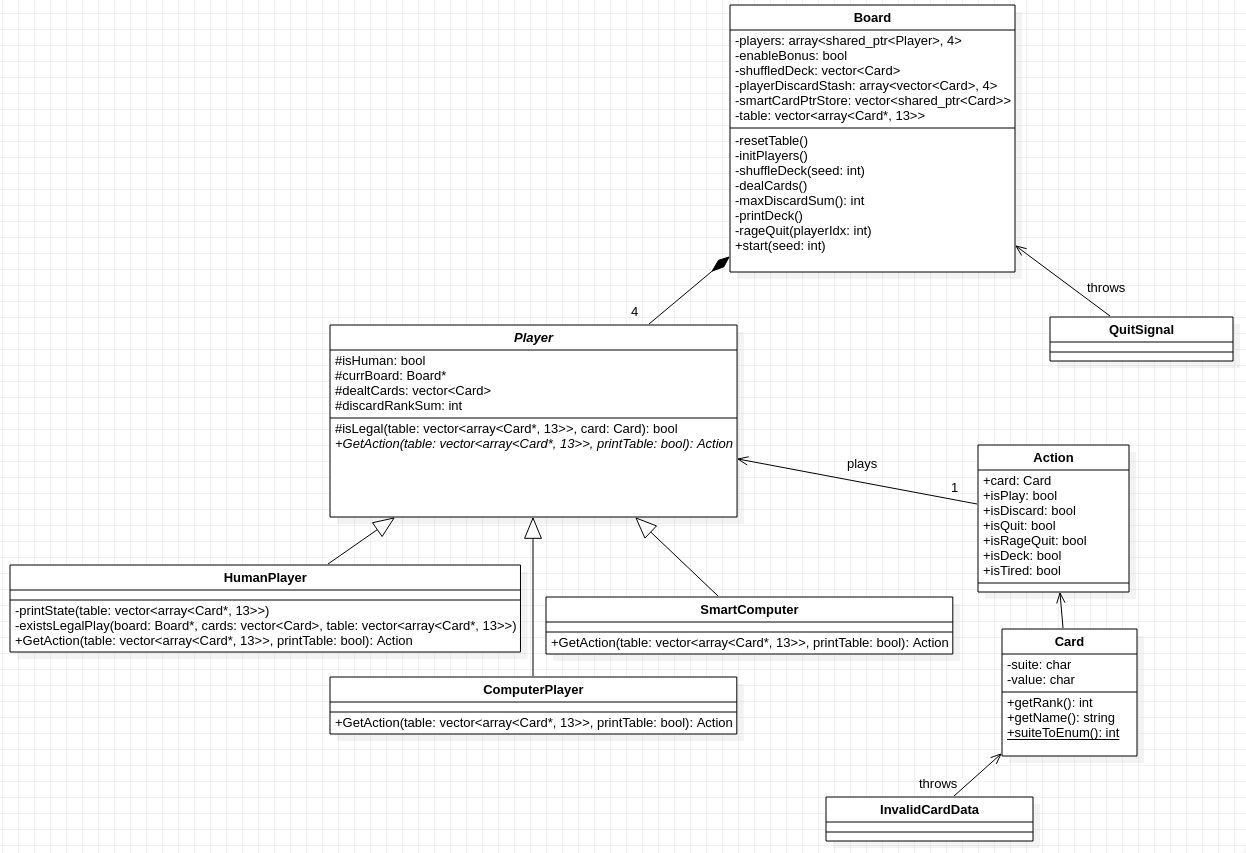
\includegraphics[width=\textwidth]{../UML/uml-final.png}
		\end{figure}
		You can reference the UML diagram above for more information about the relationships between classes.

		Since this is a card game, I first worked on a Card class which used accessors and mutators to restrict the cards' suite and value to be valid (e.g.\ a ``0 of hearts'' cannot exist). I also built an empty \texttt{InvalidCardData} class for use in throwing more descriptive exception in the cases of invalid card data.
		Next, the \texttt{Action} class represents any possible action a player of the game may want to play. This action class is quite simple: a set of booleans representing the user's selected command and a \texttt{Card} field if the user specifies a specific card (e.g.\ to play or discard).

		The \texttt{Player} class uses the decorator design pattern and is an abstract base class which is decorated by various types of players. The Player class creates a minimal structure common among all types of players, and then the classes \texttt{HumanPlayer}, \texttt{ComputerPlayer}, and \texttt{SmartComputer} are subclasses of \texttt{Player} which decorate upon it. The \texttt{Player} class specifies a virtual ``\texttt{getAction}'' method, which is used to enable communicate between the user, \texttt{Player} class, and \texttt{Board} class.

		The \texttt{Board} class can be considered the controller of the game as it handles most of the logic and handling of other classes to execute the game. The players are initialized in \texttt{Board}'s initialization process, and the seed is passed to the \texttt{Board.start} method which is effectively the handler for the game as a whole. The relationship between players uses the Observer design pattern (especially when it comes to the ``\texttt{imtired}'' command which will be covered later in this document) where other players are provided change notifications through the \texttt{Board} class. Here, the \texttt{Player} acts as a concrete observer while the \texttt{Board} acts as the subject. Since I built the program to follow RAII principles, instead of handling memory during the quit sequence, I made an empty \texttt{QuitSignal} class and threw it as an exception. I caught that exception in the main function to end the program without unintended side-effects.

	\section{Design}
		As mentioned in the previous section I used design patterns to my advantage to simplify the design. The design was inspired by the way people play card games in real-life. I thought about the ownership of the different elements of card games if I were to play Straights in real life. Through this approach, I was able to determine an intuitive class relationship model and base my design approach on that.

		One challenge I had was the co-dependency of \texttt{Board} and \texttt{Player.} I found the original structure of the project led to a recursive dependency between the two classes in which pre-compiler flags were not of help. To solve the issue I expanded the number of options in the \texttt{Action} class and had the \texttt{Player.getAction} method release more information and become more specialized in it's task: from an \texttt{Action} handler to simply fetching a valid \texttt{Action} from the player. The helped as \texttt{Board} could call \texttt{Player.getAction,} provide the information as parameters and make the relationship one-way. Through this technique, I was able to remove most of \texttt{Player}'s dependence on \texttt{Board}, and forward declare the \texttt{Board} class rather than \texttt{\#include} the code in \texttt{Player}.
		Encountering this issue really solidified the concept of minimizing coupling, as I experienced the impact of a high degree of coupling and had to redo my approach to lower the degree of coupling in between my classes.

		{\bf Changes from Due Date 1}: My design as reflected by the UML diagrams has retained the general structure from due date one to two. The three class changes are the removal of the \texttt{Deck} class and addition of \texttt{QuitSignal} and \texttt{InvalidCardData} classes. I initially intended the \texttt{Deck} class to act as a front-end of sorts to a vector of \texttt{Card}s. Early in the code development process I realized that having a \texttt{Deck} class was simply unnecessary complexity as vectors of cards were already developer-friendly and provided all the methods needed for manipulation; so I scrapped the \texttt{Deck} class from my plan. When testing my code for robustness and bugs, I realized having descriptive exceptions would not only be useful in the debugging process, but could help with managing the call stack and managing edge cases appropriately. This led to the decision to create the empty classes \texttt{QuitSignal} and \texttt{InvalidCardData} for the use of exception handling. Additionally I added a lot of new methods and fields to my plan between due date 1 and 2. Honestly, I initially underestimated the complexity of this project and expected relatively few distinct issues to take care of, which led to a simplistic class design. As I worked on the project, I found the need for better distribution of responsibilities, and thus created new methods to follow those principles.
	\section{Resilience to Change}
		From the start of the project I knew I wanted to work on extra credit features but wasn't sure which ones I'd end up implementing; so I was effectively forced to write code in a way that accommodates for change.

		Because of the modular design of the project, most changes only need to be reflected in one portion of the code, rather than looking for code to change and then hunting for bugs. For example, if the rules about which cards are legal plays changed, I could simply update the algorithm in the \texttt{Player.isLegal} method. If the handling of user actions changed, only the \texttt{Board.start} method would need to be updated. If one wanted to create a new command, I would need to add one boolean field to the \texttt{Action} class, add the user request process in \texttt{Player.getAction}, and handling in \texttt{Board.start}. Since there is only one place for each step/process, it is clear from the beginning where changes need to be reflected and what changes to make in different sections.

		This design relied heavily on a high degree of class cohesion, which led to significant clarity regarding the responsibilities of various methods and classes.

		A real-life example is the ``\texttt{imtired}'' command. As a part of the extra credit features, I decided to implement a new command after the base program was complete. Making the changes took me 20 minutes since there was already a clear structure for the development and handling of commands.
	\section{Answers to Questions}
		{\bf Question}: What sort of class design or design pattern should you use to structure your game classes so that changing the interface or changing the game rules would have as little impact on the code as possible? Explain how your classes fit this framework.\\
		{\bf Answer}: The majority of game handling is being done in the {\tt Board} class, while the process of getting the moves will be handled by the {\tt Player} class. Such a structure allows the rules to be set in a clearly defined part of the code, while each class can refer to those rules through methods, allowing for extendability. For example, if we were to allow cards with rank 6 to be played without a neighbouring ranked card of the same suite (instead of 7), this can become a one-digit change in the implementation of {\tt Player::isLegal}. Since Player is an abstract class, such a change would be propagated down to the subclasses, leading to minimal changes in the codebase.\\
		{\bf Changes from Due Date 1}: Instead of spreading the rules among different classes, I unified them to make changing rules easier. Additionally, I clarified the effect of changes on the \texttt{Player} class on subclasses.
		\\\\
		{\bf Question:} If you want to allow computer players, in addition to human players, how might you structure your classes? Consider that different types of computer players might also have differing play strategies, and that strategies might change as the game progresses i.e.\ dynamically during the play of the game. How would that affect your structure?\\
		{\bf Answer}: Referring to the UML diagram, computer players are represented as child classes of a generic {\tt Player} class with a virtual {\tt getAction} method. This method will be overridden in the implementation of the various non-human Player subclasses with various algorithms. Since players (both computer and human) have access to the table through a parameter, they can adapt their logic (and therefore strategy) in the {\tt Player::getAction} method by simply reading the state of the table, and adjusting the Action based on the table's state.\\
		{\bf Changes from Due Date 1}: Clarified the case of multiple computer-player classes.
		\\\\
		{\bf Question}: If a human player wanted to stop playing, but the other players wished to continue, it would be reasonable to replace them with a computer player. How might you structure your classes to allow an easy transfer of the information associated with the human player to the computer player?\\
		{\bf Answer}: In the case where a human player wanted to stop playing while keeping the game running (i.e.\ ragequit), this design allows for a relatively easy switch from a code design perspective. Since any (human) player's state is uniquely identified (relative to other players) by {\tt dealtCards} and {\tt discardRankSum}, that person's {\tt HumanPlayer} object can be deleted and replaced with a {\tt ComputerPlayer} or {\tt SmartComputer} object where the {\tt dealtCards} and {\tt discardRankSum} attributes of the {\tt ComputerPlayer} set to original values (from the human who ``ragequit''). Then, this new {\tt Player} object can be reflected in {\tt Board::players}.\\
		{\bf Changes from Due Date 1}: Included case of the new {\tt SmartComputer} class.
	\section{Extra Credit Features}
		I worked on four extra credit features:
		\begin{enumerate}
			\item Completed entire project, without leaks, and without explicitly managing my own memory.
				\begin{itemize}
					\item This extra feature would have been significantly more difficult had I built the basic project first, then implemented this. Instead, I intentionally relied on RAII principles from the start and used smart pointers when I had to allocate memory in the heap.
				\end{itemize}
			\item A new command: ``\texttt{imtired}''
				\begin{itemize}
					\item When I was testing my code for bugs, I found the game to take really long to play with the 80 point minimum to end the game. The only options I had were to quit the game, or \texttt{ragequit}; neither of which allowed me to end the game on a quicker schedule. I considered lowering the score limit, but that solution would translate well to dynamic changes during gameplay.
						I came up with the idea of the ``\texttt{imtired}'' command. When a player issues the ``\texttt{imtired}'' command, all other human players are asked if they would like to end the game after the completion of the current round. If all players agreed, the player with the lowest score would be declared winner at the end of the round.
						I found this extra credit feature especially difficult to solve, first because of having to notify all other players of the poll to end the game this round. The other issue was the abundance of edge cases in this feature.
						I solved the first problem by leveraging an Observer design pattern, and using the \texttt{Board} class to store the poll state. I solved the edge case issue by making a tree diagram of the various potential poll states, accounting for each of them, and thoroughly testing the feature.
				\end{itemize}
			\item Smarter Computers
				\begin{itemize}
					\item After playing a few games of Straights, I discovered a simple but effective algorithm for selecting efficient plays and discards. If there is a legal play, play the card with the highest rank. If there is no legal play, discard the card with the lowest rank.
						Implementing this bonus feature was surprisingly simple because of the Decorator design pattern. I simply made a \texttt{SmartComputer} class which inherited from \texttt{Player}, and then built out the \texttt{SmartComputer.getAction} method. Then, I made a few changes in the \texttt{Board} class to select the appropriate computer player level based on the \texttt{--enablebonus} flag when launching the program.
				\end{itemize}
			\item Better printing and user experience
				\begin{itemize}
					\item This one is a relatively simple improvement to the user experience of playing the game.
						When I played Straights, all the commands were one after another, leading to a very cluttered and confusing terminal.
						I simply added spacing between player turns, and a header for the current player. Though simple, this change greatly improves the user experience when playing the game, and makes the player change process a lot simpler from the user's perspective. I solved this by modifying the \texttt{Board.start} method to print newlines between turns, and print the player number prior to the action selection prompt.
				\end{itemize}
		\end{enumerate}
	\section{Final Questions}
		{\bf Question}: What lessons did this project teach you about developing software in teams? If you worked alone, what lessons did you learn about writing large programs?\\
		{\bf Answer}: I worked alone on this project. The primary thing I learnt about developing large programs was organization and time-management. Luckily, I organized the code for this project neatly, which made the development process significantly easier than if I hadn't. One method of organization was using the git tool. I made a private git repository and used the ``gitflow-workflow'' process to separate my code and test for bugs before merging into the main branch which contained all the stable code.
		\\\\
		{\bf Question}: What would you have done differently if you had the chance to start over?\\
		{\bf Answer}: I would change my approach to time management. In the start, I experienced a sort of ``writer's block,'' in which I worked on the project on a theoretical level but was nervous to begin coding. As mentioned earlier in this document, when I started coding I found some design issues. Finding these issues experientially is much more efficient than taking a theoretical approach. Therefore, if I could start over I would start coding the project slightly earlier to catch roadblocks earlier on and determine a new approach.
\end{document}

